\chapter{Background}

\section{Existing Personal Clouds}

In the last few years, we have seen how the market of cloud storage is growing rapidly. 
Despite the rush to simplify our digital lives, many of the commercial Personal Clouds
in operation today like Dropbox are \textit{proprietary}, and rely on algorithms that are
\textit{invisible} to the research community, and what is even worse, existing open source
alternatives fall short of addressing all the requirements of the Personal Cloud.
Next we discuss the existing commercial and open source solutions for the Personal Cloud, namely
Dropbox, Google Drive, Box, SugarSync and OneDrive, as commercial ones and 
SparkleShare, ownCloud and Syncany, as open source solutions.

Before beginning with Personal Cloud comparison we will introduce some important concepts
and provide definitions of the main aspects that will be analysed. To clarify, we will
classify features into the following sections:

\begin{itemize}
\item \textbf{Storage}. We will take into account features such as Personal Cloud's infrastructure or whether they use advanced techniques such as data deduplication.
\item \textbf{Sync}. In this part we will describe and analyse aspects related to file synchronisation such as P2P syncing or file versioning. 
\item \textbf{Share}. Different types of data sharing and collaboration will be considered. Including privacy-aware data sharing.
\item \textbf{Privacy}. We will analyse the type of encryption used by Personal Clouds while files are being transmitted and when they are at rest. In addition we will analyse authentication protocols and software licenses used.
\end{itemize}


\subsection{Storage}

Personal Cloud companies offer sophisticated storage services to end-users and enterprises by making use of raw storage. This \textbf{storage backend} is often provided by data center owners such as Amazon or Rackspace. However, some other Personal Clouds do have their own infrastructure and do not outsource this task.

Therefore, we can classify Personal Clouds depending on their \textbf{nature}: public, private or hybrid. We call Public Clouds the ones that whose services and infrastructure are offered off-site over the Internet. In contrast, a Private Cloud is one in which the services and infrastructure are maintained on a private network. Additionally, Hybrid Clouds include a variety of public and private options with multiple providers. For instance, a company could keep sensible and business critical information in their Private Cloud, while using a Public Cloud to store the rest of their data.

Personal Clouds usually offer their services based on a Freemium business model~\footnote{Freemium is a business model by which a product is offered free of charge, but a premium product with advanced features at a charge.}. In other words, a product is offered free of charge, but a premium product with advanced features is offered at a charge. Therefore, the storage quota offered for free is an important feature that users consider.

Some Personal Clouds apply restrictions on the \textbf{maximum file size}, which can vary depending on whether the file is synced on the desktop application or uploaded through the web interface, or even the type of account.

In order to optimize the storage and bandwidth consumed when maintaining different versions of files some Personal Clouds use \textbf{data deduplication} techniques. Using data deduplication, when a user is to upload a file that already exists in the Cloud, he will not need to actually transfer it. Instead, a logical relation between the file and the user will be created. This technique can be applied to different scopes (i.e. across all files in the system, across user's files, etc.) depending on the privacy policy.

Such popular services need to scale well in order to be successful. A system is said to be \textbf{scalable} when it is able to accommodate a significant growth in its amount of work and continue its normal functioning. This feature is normally inherited by the storage backend that underlies the service.

\begin{table}
\begin{center}
    \begin{tabular}{ | p{3cm} | p{1.8cm} | p{1.5cm} | p{2.6cm} | p{1.3cm} | p{1.5cm} | }
    \hline
    \rowcolor[gray]{0.8}

	\textbf{Personal Cloud} &
	\textbf{Nature} &
	\textbf{Free storage} &
	\textbf{File size limit} & 
	\textbf{Dedup.} & 
	\textbf{Scalable} \\ \hline

	\textbf{Google Drive} &
	Private &
	5 GB &
	10 GB &
	No &
	Yes \\ \hline

	\textbf{Dropbox} &
	Public (Amazon S3) &
	2 GB &
	300 MB (web only) &
	Yes &
	Yes \\ \hline
	
	
	\textbf{Box} &
	Private &
	5 GB & 
	250 MB (free acounts) &
	? &
	Yes \\ \hline
	
	\textbf{SugarSync} & 
	Public (Carpathia Hosting) &
	5 GB &
	Unlimited &
	? &
	Yes \\ \hline
	
	\textbf{OneDrive} & 
	Private &
	7 GB &
	2 GB (client), 300 MB (web) &
	? &
	Yes \\ \hline
	
	\textbf{ownCloud} &
	Private &
	Custom &
	Custom &
	No &
	No \\ \hline

    \end{tabular}
    \\[10pt]
    \caption{Personal Cloud comparison on storage features}
    \label{tab:pc_storage}
\end{center}
\end{table}

As we can see in table~\ref{tab:pc_storage}, most of the analysed Personal Clouds use their own storage backend, others such as Dropbox or Ubuntu One rely on well-known storage providers such as Amazon to store users' data. Most Personal Clouds allow users to increase their free storage by referring friends to their service. We can also observe that there is a huge difference on the limit set to file sizes. OwnCloud lets administrators assign custom values for storage space and file size limit.

\subsection{Sync}
One of the key aspects of Personal Clouds is \textbf{file synchronization} (or syncing). We understand it as a two-way file synchronization, which means that a locally modified file is updated in each location this file is present. In addition, if a file is modified remotely, these changes will be automatically updated locally, with the purpose of keeping every copy of a file identical in all locations.

Another interesting feature is \textbf{versioning}. File versioning allows users to restore previous versions of a file. Personal Clouds may limit the \textbf{version history} to a maximum number of revisions to be kept in the system or a specific period of time. For instance, a company could claim storing all versions of a file done in the last 30 days. This may also vary depending upon whether it is a free account or not.


{
\def\arraystretch{1.5}

\begin{table}
\begin{center}
    \begin{tabular}{ | p{3.3cm} | p{2cm} | p{2.9cm} | }
    \hline
    \rowcolor[gray]{0.8}

	\textbf{Personal Cloud} &
	\textbf{Versioning} & 
	\textbf{Versions saved} \\ \hline

	\textbf{Google Drive} &
	Yes &
	30 days or 100 versions \\ \hline

	\textbf{Dropbox} &
	Yes &
	30 days \\ \hline
	
	\textbf{Box} &
	Yes &
	10 \\ \hline
	
	\textbf{SugarSync} & 
	Yes &
	2 (free), 5 (paid) \\ \hline
	
	\textbf{OneDrive} & 
	Yes &
	25 \\ \hline
	
	\textbf{ownCloud} &
	Yes &
	? \\ \hline

    \end{tabular}
    \caption{Personal Cloud comparison on syncing features}
    \label{tab:pc_syncing}
\end{center}
\end{table}
}

\subsection{Share}


Sharing is an attractive feature that most of Personal Clouds provide, whether it is with users inside the service or with people outside the Personal Cloud. \textbf{Internal sharing} is usually offered as an integrated functionality in the user interface. Whereas \textbf{public sharing} is commonly offered as direct HTTP links that allow other users to access to certain files or folders.


{
\def\arraystretch{1.5}

\begin{table}
\begin{center}
    \begin{tabular}{ | p{3.3cm} | p{1.5cm} | p{2cm} | p{2.5cm} | }
    \hline
    \rowcolor[gray]{0.8}

	\textbf{Personal Cloud} &
	\textbf{Internal sharing} &
	\textbf{Public file sharing} &
	\textbf{Collaborative editing} \\ \hline

	\textbf{Google Drive} &
	Yes &
	Yes &
	Yes \\ \hline

	\textbf{Dropbox} &
	Yes &
	Yes &
	No \\ \hline
	
	\textbf{Box} &
	Yes &
	Yes &
	No \\ \hline
	
	\textbf{SugarSync} & 
	Yes &
	Yes &
	No \\ \hline
	
	\textbf{OneDrive} & 
	Yes &
	Yes &
	Yes \\ \hline
	
	\textbf{ownCloud} &
	Yes &
	? &
	No \\ \hline

    \end{tabular}
    \caption{Personal Cloud comparison on sharing features}
    \label{tab:pc_sharing}
\end{center}
\end{table}
}

As we can see in table~\ref{tab:pc_sharing}, only Google Drive and OneDrive let multiple users collaborate simultaneously on the same file from any computer. When someone makes changes to a document, the other person can see the changes in real-time and respond to the edits immediately.

\subsection{Privacy}


Personal Clouds must ensure that user data is not accessed by third-parties and only authenticated users are granted access. Some companies use standard \textbf{authentication protocols} such as OAuth~\cite{oauth}, others opt for using their own mechanisms.

As a security measure, some companies store user data encrypted. Many Personal Clouds can provide \textbf{server-side encryption}; meaning that users delegate to the Cloud the task of protecting their files and managing their keys. As an alternative, \textbf{client-side encryption} allows users to encrypt their data before it is transmitted to the server. So the user is responsible for managing the keys and the service provider is unable to decrypt their data, adding an extra layer of security.

Besides the fact of having the files secured when they are at rest in the server, it is also essential to assure their privacy when they are being transmitted to and from the server. Personal Clouds usually use \textbf{HTTPS} to communicate to their services either from the desktop application or other tools such as the REST APIs or the web interface.


{
\def\arraystretch{1.5}

\begin{table}
\begin{center}
    \begin{tabular}{ | p{3.3cm} | p{2.5cm} | p{2.2cm} | p{2.2cm} | p{2cm} | }
    \hline
    \rowcolor[gray]{0.8}

	\textbf{Personal Cloud} &
	\textbf{Authorization protocol} &
	\textbf{Client-side encryption} &
	\textbf{Server-side encryption} & 
	\textbf{Secure channel (HTTPS)} \\ \hline
	
	\textbf{Google Drive} &
	OAuth 2.0 &
	No &
	No &
	Yes \\ \hline

	\textbf{Dropbox} &
	OAuth 1.0 &
	No &
	Yes (AES 256-bit) &
	Yes \\ \hline
	
	\textbf{Box} &
	OAuth 2.0 &
	No &
	Yes (AES 256-bit) &
	Yes \\ \hline
	
	\textbf{SugarSync} & 
	Custom. Token-based &
	No &
	Yes (AES 128-bit) &
	Yes \\ \hline
	
	\textbf{OneDrive} & 
	OAuth 2.0 &
	No &
	Yes &
	Yes \\ \hline

	
	\textbf{ownCloud} &
	--- &
	No &
	Yes &
	Yes \\ \hline

    \end{tabular}
    \caption{Personal Cloud comparison on privacy features}
    \label{tab:pc_privacy}
\end{center}
\end{table}
}

As we observe in Table~\ref{tab:pc_privacy}, most Personal Clouds implement the OAuth protocol on their API services, either the 1.0 or 2.0 version. Others like SugarSync use their own authentication mechanisms. In general terms, a user makes a call providing his credentials to obtain a refresh token. Next, the user will use this refresh token to obtain an access token that will grant access to the user's resources. As the access token has an expiry date, the user will have to use the refresh token periodically to extend its lifetime.

None of the Personal Clouds provide built-in client-side encryption. Unanimously, all services establish a secure channel between user's computer and the storage provider before data is transmitted. That way, no one can eavesdrop on the transfer.

\section{Open Source Personal Cloud Systems}

After studying the state-of-the-art of the exisiting Personal Clouds, we discuss in more detail
the existing open source solutions.

\subsection{SparkleShare}

SparkleShare\footnote{\url{http://sparkleshare.org/}} is built on top of Git, using it 
as both its storage and syncing back-end. SparkleShare clients use push notification
to receive changes, and maintain a direct connection with the server over SSH to exchange file data.
When a client is started, it connects to a notification server. The notification server tells the other
clients subscribed to that folder that they can pull new changes from the repository after a user
change. 

Using Git as the storage back-end is a double-edged sword. While Git implements an efficient request
method to download changes from the server (git pull command), avoiding massive metadata exchanges
between server and clients, it is not prepared to process large binary files. Also, this architecture
tied to the Git protocol is also difficult to scale and deploy in cloud environments.

\subsection{ownCloud}
ownCloud\footnote{\url{http://owncloud.org/}} is the most famous open source  Personal Cloud 
and they have an active community. We refer here to the Community Edition of ownCloud, since their enterprise edition is not available to the public. In ownCloud, clients communicate with the server following a \textit{pull} strategy, i.e. clients ask periodically to the server for new changes. There are two types of data traffic: data and metadata. For data exchange, ownCloud uses a REST API; however, metadata traffic is transferred using the WebDAV protocol. 
Because both types of traffic are processed by the same server, data and metadata traffic are completely coupled.

Unfortunately, ownCloud is not an extensible and modular framework like StackSync. In this line, their developer community is mainly working around the web front-end. Although we will devote a subsection to ownCloud in the validation, we can advance that their inefficient pull strategy with massive control overheads is not scalable. Furthermore, their sync flows and data flows are tightly coupled, and they do not even provide basic chunking or deduplication mechanisms. 

\subsection{Syncany}
Syncany \footnote{\url{http://syncany.org/}} is an open source Personal Cloud developed by Philipp Heckel in Java. It is a client-side Java application that can synchronise against a variety of storage back-ends thanks to their extensible plugin model. They also provide extensible mechanisms for chunking and their architecture is elegant, clean and modular.

Although we give much credit to Syncany, proof of that is that the StackSync client is a branch project that evolved 
from Syncany, it presents a number of drawbacks that made us evolve towards the current StackSync architecture. 
The major shortcoming is the lack of scalability of Syncany due to its heavy pull strategy with metadata and
data flows heavily coupled. To support versioning and resolve conflicts, Syncany relies on a metadata file 
that contains the complete history of each individual file, and that is stored in the storage back-end
as a regular file. To determine the most recent version of a file, the Syncany client needs first to
download this metadata file, which grows with each new file modification, severely limiting scalability.

\subsection{What to choose?}
As explained before, none of the current open source solutions fits well in a Personal Cloud definition.
For this reason, we decided to create StackSync, an open framework for Personal Cloud systems. Its architecture is
highly modular, with each module represented by a well-defined API, allowing third parties to replace components
for innovation in versioning, deduplication, live synchronization or continuous reconciliation, among other
relevant topics.

\section{StackSync}

\lstset{language=Java,
basicstyle=\ttfamily\footnotesize,
keywordstyle=\color{javapurple}\bfseries,
stringstyle=\color{javared},
commentstyle=\color{javagreen},
morecomment=[s][\color{javadocblue}]{/**}{*/},
numbers=left,
numberstyle=\footnotesize\color{black},
stepnumber=1,
numbersep=10pt,
backgroundcolor=\color{black!5},
frame=single,
tabsize=4,
showspaces=false,
showstringspaces=false}


In general terms, StackSync can be divided into four main blocks: clients, synchronization service, storage service, and communication middleware. An overview of the architecture with the main components and their interaction is shown in Figure~\ref{fig:architecture}. The
StackSync client and the sync service interact through the communication middleware called ObjectMQ. The sync service interacts with the
metadata database. The StackSync client directly interacts with the storage
back-end to upload and download files.

\begin{figure}[h]
\centering
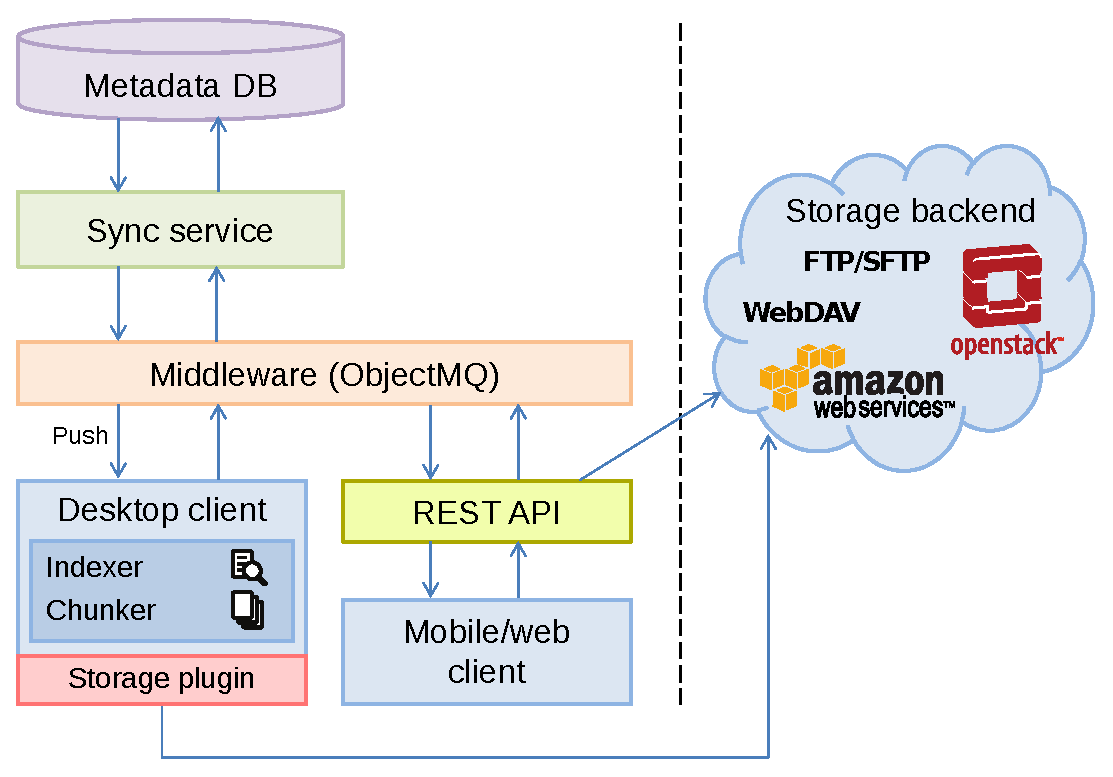
\includegraphics[width=0.55\textwidth]{figures/big_picture_v2}
\caption{StackSync architecture overview}\label{fig:architecture}
\end{figure}

As we can see in the figure above, the storage back-end is separated from the rest of the architecture by a line. This means that StackSync can be used with external storage back-ends such as Amazon S3 or RackSpace. This enables StackSync to fit different organization requirements and be offered in three different configurations:

\begin{itemize}
\item \textbf{Public Cloud.} Data and metadata is stored in a public storage provider such as Amazon or Rackspace.
\item \textbf{Private Cloud.} StackSync is installed on-premise. Data and metadata is stored on the company’s infrastructure.
\item \textbf{Hybrid Cloud.} Data is stored in a public storage provider and metadata is kept inside the company’s infrastructure.
\end{itemize}

\subsection{StackSync Synchronization Protocol}

Since file synchronization lies at the heart of any Personal Cloud service, 
we present a reference synchronization protocol that is available in the StackSync framework,
which is based on a \textit{message-oriented middleware} (MOM). In particular, 
MOM is ideally suited here for:

\begin{enumerate}
\item \textit{Scalable change notification:} The high read-write ratio of Personal Cloud services makes
it more appropriate to employ \textit{one-to-many push communication} for quickly notification.  
Server-based protocols like this are required when replicas need a high degree of consistency \cite{Tanenbaum:2001:DSP:559404}.
\item \textit{Asynchronous message dispatching:}  Synchronization operations require significant
server processing time for ensuring consistency. Decoupling message dispatching from message
processing in these scenarios  \cite{menasce2005mom} is important for scalability reasons.
\item \textit{Implicit load balancing:} When many consumers read from a queue, messages are
distributed among them. This way, we can start multipe
instances of the \texttt{SyncService} to alleviate the load of the incoming request queue,
\textit{allowing to scale up and down very easily as computing needs change}.
\end{enumerate}


\subsection{Desktop client and Storage back-ends}

The main StackSync client is a application that monitors local folders and synchronizes them with a remote repository. The StackSync client interacts with both the synchronization and storage services. The first one handles metadata communication, such as time stamps or file names, and the second one is in charge of raw data.


This decoupling of sync control flows from data flows implies a user-centric design where the client directly controls its digital locker or storage container. The synchronization protocol have been designed to put the load in the client side, whereas the synchronization service just
checks if the change is consistent, and then applies all changes proposed by clients.


Every client has a local database and a process called \texttt{Watcher} that is responsible for monitoring the state of local folders that have been selected to be synchronized. If there is any change in the local repository, the \texttt{Watcher} notifies a process called \texttt{Indexer} which is responsible for sending these changes to the synchronization service. Besides that, the \texttt{Indexer} can also receive events from the synchronization service indicating that there was a change in the remote repository. These notifications are applied immediately into the local repository. Regarding potential
conflicts due to offline operations, StackSync provides similar policies than Dropbox, so that we create a copy of the conflicted document and let the user decide about this.


The client uses a chunking algorithm to split files into chunks before they are transmitted to the storage service. To save storage space and bandwidth, the StackSync client uses data deduplication at the chunk level so it only stores and transmits those chunks that have not been uploaded before. 


Finally, and based on the original Syncany architecture, we provide an extensible plugin-based architecture for connecting to third-party Storage back-ends. We now provide plugins for Amazon S3, OpenStack Swift, Dropbox, WebDAV, SMB and FTP. However, we are focusing our efforts on OpenStack Swift, a highly available, distributed, eventually consistent object/blob store that guarantees service scalability.


\subsection{Communication middleware}

StackSync relies on a high-performance message broker compatible with the Advanced Message Queueing Protocol (AMQP)~\cite{amqp} standard. In order to simplify the interaction with this messaging middleware, we have built the ObjectMQ communication middleware.


ObjectMQ is a lightweight remote object layer constructed on top of a messaging
middleware. The current StackSync implementation relies on RabbitMQ, an open source message broker software that implements the AMQP standard. ObjectMQ combines RPC (Remote Procedure Call) and MOM (Message-oriented Middleware) models to devise four MOM-RPC invocation abstractions: two one-to-one calls (synchronous, asynchronous) and two one-to-many calls (multi, event).


In general, objects receive method calls as messages in incoming queues, and then reply the results to clients in response queues. One-to-many calls are distributed using the appropriate AMQP Exchanges (broker message dispatchers). Recall that Exchanges determine message delivery and provide different delivery schemes, like direct (deliver this message to a particular queue) and publish-subscribe (deliver this message to all queues subscribed to a certain topic). 

These are the four available calls:

\begin{itemize}

\item @async:  This is an asynchronous non-blocking  one-way invocation where the client  publishes a message in the target object request 
Queue ($Q_{Request}$). By default, the client expects to receive no response and it is even not notified if the message was handled correctly.


\item @sync:  This is a synchronous blocking remote call where the client publishes a message in the target object
request Queue ($Q_{Request}$), blocking until a response is received in its own client response queue ($Q_{Response}$).  
This call can be configured with a timeout and a number of retries to trigger the exception if the result does not arrive.

\item @event:  This is an asynchronous non-blocking one-to-many notification triggered by a server.  The server triggers an @event by publishing the message in  the Event  fan-out Exchange ($E_{Event}$). Any client subscribing to this event in the server must bind their incoming Event Queue ($Q_{Event}$) to the server Exchange ($E_{Event}$).

\item @multi: This is an asynchronous non-blocking one-to-many invocation from one client to many servers. The clients invokes the method in all servers by publishing an event in the Multi  fan-out Exchange ($E_{Multi}$). All servers bind their incoming Request Queue ($Q_{Request}$) to the Multi Exchange ($E_{Multi}$).
   
\end{itemize}

The ObjectMQ communication middleware supports different compression and transport protocols (Kryo~\cite{kryo}, Java Serialization, JSON). It also handles transparently all the error management and communication services on top of the MOM broker. By creating this middleware, that the initial code of the StackSync client has been reduced in around $3,000$ lines of code.


\subsection{Synchronization service and metadata back-end}

The Sync service is a server-side component implemented as a remote object using the ObjectMQ communication middleware. This service directly benefits from the invocation abstractions offered by ObjectMQ. 

\begin{figure}[t]
\centering
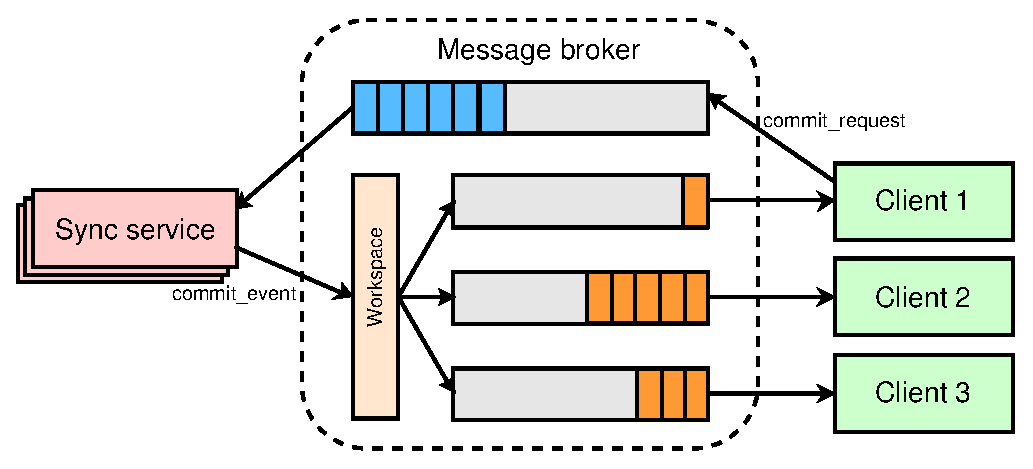
\includegraphics[width=0.66\textwidth]{figures/message_broker}
\caption{Message broker communication flow}\label{fig:message_broker}
\end{figure}


In Figure~\ref{fig:message_broker} we can observe the current design, ObjectMQ is using a global request queue for the SyncService, 
a response queue for each device (Sync service Proxy), and a fan-out Exchange for each workspace.  

Each device will bind its request queue to the appropriate workspace Exchange to receive notification changes in this workspace.  In any case, queue message programming is abstracted thanks to ObjectMQ, so that the protocol will be defined in terms of RPCs or method calls.


\bigskip
\begin{figure}[h!]
	\begin{lstlisting}
	@RemoteInterface
	public interface SyncService extends Remote {

    	@SyncMethod(retry = 5, timeout = 1500)
    	public List<ObjectMetadata> getChanges(Workspace workspace);

    	@SyncMethod(retry = 5, timeout = 1500)
    	public List<Workspace> getWorkspaces();

    	@AsyncMethod
    	public void commitRequest(Workspace workspace, 
    		List<ObjectMetadata> objectsChanged);

	}
	@event
	public interface CommitEvent extends Event {
		
		public List<ObjectMetadata> objectsChanged getChanges();
	}
	
		\end{lstlisting}
		\caption{Sync service interface}
		\label{fig:idl}
\label{Code:push}
\vspace{-10pt}
\end{figure}


In Figure~\ref{fig:idl} we can see the interface definition of the Sync service. Clients can request the list of Workspaces they have access to with the \texttt{getWorkspaces} operation. Once the client obtains the list of Workspaces, it can then perform two main operations: \texttt{getChanges} and  \texttt{commitRequest}. Furthermore, the client will be notified of changes  by means of the event \texttt{CommitEvent}.

\texttt{getChanges} is a synchronous operation (@sync) that StackSync clients perform on startup. This is a costly operation for the Sync service as it returns the current state of a Workspace. Once the client receives this information, it registers its interest in receiving committed updates (i.e. \texttt{CommitEvent}s (@event) for this Workspace). From that point on, any change occurring on this Workspace will be notified to the client in a push style.

\texttt{commitRequest} is an asynchronous operation (@async) that clients employ to inform the Sync service about detected file changes in their Workspaces.  This is a  costly operation since it must guarantee the consistency of data after the new changes. 

\texttt{CommitEvent} is triggered by the Sync service in an asynchronous one-to-many operation (@event) to all out-of-sync devices in the specified Workspace. This operation is only launched by the Sync service once the changes has been correctly stored in the \texttt{Metadata back-end}.

\begin{algorithm}[h]
  \caption{Pseudocode of the commitRequest function in the Sync service}
    \label{alg:commit_pseudocode}
  \begin{algorithmic}[1]
  	\footnotesize
    \Function{commitRequest}{$workspace, List<ObjectMetadata> objects\_changed$}
      \State $commit\_event \gets $ new instance of CommitEvent
      \For{$new\_object$ \textbf{in} $objects\_changed$}
      	\State $server\_object \gets metadata\_backend.get\_current\_version(new\_object.id)$
        \If {\textbf{not exists} $server\_object$}
          	\Comment To commit the first version of the new object
        	\State $metadata\_backend.store\_new\_object(new\_object)$
        	\State $commit\_event.add(new\_object, \mathtt{confirmed} = True)$
        \ElsIf{$server\_object.version$ \textbf{precedes} $new\_object.version$}
         	\\ \Comment No conflict, committing the new version
			\State $metadata\_backend.store\_new\_version(new\_object)$
			\State $commit\_event.add(new\_object, \mathtt{confirmed} =True)$
        \Else
        	\\
        	\Comment Conflict detected, the current object metadata is returned
        	\State $commit\_event.add(new\_object, \mathtt{confirmed} = False,  server\_object)$
        \EndIf
      \EndFor 
      \State $trigger\_event(workspace, commit\_event)$
    \EndFunction
  \end{algorithmic}
\end{algorithm}


Algorithm~\ref{alg:commit_pseudocode} reports the pseudocode of the \texttt{commitRequest} operation. When a \texttt{commitRequest} message is received in the global request queue, the ObjectMQ middleware will invoke the appropriate \texttt{commitRequest} method in the \texttt{SyncService}. 


This method then receives a proposed list of change operations in a concrete Workspace. For every change operation, it will then check if the current version of the object in the \texttt{Metadata back-end} precedes the change proposed by the client. In this case, the changes are (transactionally) stored in the Metadata back-end and confirmed in the \texttt{CommitEvent}. 

If there is a conflict with versions, the \texttt{commitRequest} is set as failed and information about the current object version is added to the \texttt{CommitEvent}. The reason for adding the current object version to the \texttt{CommitEvent} is to piggyback the information about the ``differences'' between the two versions, such that the ``losing'' client can identify the missing chunks and reconstruct the object to the current version. 


In StackSync, a conflict may occur when two users change a file at the same time. This implies that the two clients will propose a list of changes over the same version of the file. The first \texttt{commitRequest} to be processed will
increase the version number by one, but the second \texttt{commitRequest} will inevitably propose a list of changes over a preceding version, resulting in a conflict. 

To resolve the conflict, the Sync service adopts the simplest policy in this case, which is to consider as the ``winner''  the client whose \texttt{commitRequest} was processed first. This way, the Sync service
avoids rolling back any update to the Metadata back-end, saving time and increasing scalability. At the client,
the conflict is resolved by renaming the ``losing'' version of the file to ``...(conflicted copy)''.

Finally, the \texttt{CommitEvent} will be triggered to the Workspace Exchange in message broker, and  it will be received by all interested devices in their incoming event queues. 

Note that the \texttt{CommitRequest} is an important operation in the Sync service since it has to provide scalable request processing, consistency, and scalable change notification. Scalable request processing is achieved because the method is \textit{asynchronous} and \textit{stateless}. Multiple Sync service instances can listen from the global request queue and the message broker will transparently
balance their load. Consistency is achieved using the transactional  ACID model of the underlying Metadata back-end. 
Finally, scalable change notification to the interested parties is achieved using one-to-many push notifications (@event).

The Sync service interacts with the Metadata back-end using an extensible DAO (Data Access Object). Our reference implementation is based on a PostgreSQL relational database although the system is modular and may be replaced easily.